% !TEX encoding = UTF-8 Unicode
% LaTeX file for resume 
% This file uses the resume document class (res.cls)

\documentclass{res} 
\usepackage{fontspec}
\usepackage{tikz}
\usepackage{xeCJK}
\usepackage{listings}
\usepackage[autostyle]{csquotes} 
\usepackage{hyperref}

\lstset{
	language=C,
	numberstyle=\footnotesize,
	basicstyle=\footnotesize\ttfamily,
	numbers=left,
	stepnumber=1,
	frame=shadowbox,
	breaklines=true,
	postbreak=\raisebox{0ex}[0ex][0ex]
		{
			\ensuremath{\color{red}\hookrightarrow\space}
		}
}
% lstlisting tree command
\lstdefinestyle{ascii-tree}{
    literate={├}{|}1 {─}{--}1 {└}{+}1 
}
  
\setCJKmainfont{STHeiti} % chinese type
%\setCJKmainfont{BiauKai}
%\usepackage{helvetica} % uses helvetica postscript font (download helvetica.sty)
%\usepackage{newcent}   % uses new century schoolbook postscript font 
\setlength{\textheight}{9.5in} % increase text height to fit on 1-page 
\usepackage{enumitem}

\XeTeXlinebreakskip = 0pt plus 1pt 

\begin{document} 


\name{\LARGE Real Time System Project2 Report}     % the \\[12pt] adds a blank
				        % line after name
\address{\\R03922106 蔡佑隆 unzledick@yahoo.com.tw\\ R04922067 楊翔雲 morris821028@gmail.com}

\begin{resume}

\vspace*{.1in} \noindent {\large \bfseries 作業描述}

	修改 linux kernel,在 \lstinline{kernel/sched.c} 相關 scheduler 部分增加 Weighted Round-Robin scheduler、Shortest Job First scheduler 以及 Rate-monotonic scheduler。最後藉由 Project 1 的練習撰寫測試程序驗證 scheduler 是否符合預期結果。

\vspace*{.1in} \noindent {\large \bfseries 測試環境}

\begin{itemize}
	\item Ubuntu 14.04.3 LTS (GNU/Linux 3.13.0-62-generic x86\_64)
	\item qemu-system-x86\_64
\end{itemize}


\vspace*{.1in} \noindent {\large \bfseries 環境安裝}

參閱附錄 \lstinline{README.md}

\vspace*{.1in} \noindent {\large \bfseries 修改檔案列表}

\begin{lstlisting}[style=ascii-tree]
.
├── README.md
├── arch
│   └── x86
│       ├── include
│       │   └── asm
│       │       ├── unistd_32.h
│       │       └── unistd_64.h
│       └── kernel
│           └── syscall_table_32.S
├── include
│   └── linux
│       ├── sched.h
│       └── syscalls.h
└── kernel
    ├── sched.c
    ├── sched_fair.c
    ├── sched_rt.c
    └── sched_weighted_rr.c
\end{lstlisting}


特別注意到,若編譯環境為 x86\_64 則需要額外修改 \lstinline{arch/x86/include/asm/unistd_64.h} 複製 \lstinline{arch/x86/include/asm/unistd_32.h} 增加的 syscall。 同理,增加自己定義的 syscall 時,需要修改 \lstinline{arch/x86} 下的那三個檔案 (如果發現編譯 kernel 時,出現 \lstinline{WARNING: syscall NOT IMPLEMENTION.} 大多數都是這個造成)。

在 \lstinline{include/linux/sched.h} 中,增加 task 的成員變數,提供接下來針對 task 操作需要的參數,特別的是在 \lstinline{struct sched_rt_entity;} 中,相較於一般資料結構的寫法,linux 採用倒過來將節點訊息放在資料內部中,利用 \lstinline{#define container_of(ptr, type, member)} 取得物件訊息,這種寫法方便解決 task 在數個 scheduler 中轉換。

因為 syscall 的方式設定 task weighted,增加一個全區變數 \lstinline{int weighted_rr_time_slice;},每一次 syscall 去設定這一個全區變數值,然後 task 建立時,經過 \lstinline{sched_fork},直接利用被修改全區變數作為這一個 task 的 weight。若要特別針對 task 設定 weighted round-robin,在建立前都要呼叫 syscall 設定全區變數。

\begin{lstlisting}[frame=single]
struct sched_rt_entity {
    ...
    //+ RTS Proj2: weighted_rr
    struct list_head weighted_rr_list_item;
    ...
};
...
struct task_struct {
    ...
    //+ RTS Proj2: weighted_rr
    unsigned int task_time_slice;
    //+ RTS Proj2: weighted_rr_prio
    unsigned int weighted_time_slice;
    ...
};
...
//+ RTS Proj2: weighted_rr
extern int weighted_rr_time_slice;
\end{lstlisting}

\vspace*{.1in} \noindent {\large \bfseries Source Code}

\vspace*{.05in} \hspace*{.1in} \noindent {\bfseries Part 1. Weighted Round-Robin Scheduler}

\begin{itemize}
	\item 
	\lstinline{enqueue_task_weighted_rr()} \\
	函數將會給予 task 和 rq,將 task 根據 rq 的資料結構重新將 task 放入。若按照 \lstinline{list} 結構,直接模擬 queue 即可,由於 linux 提供 list 本身為雙向串列,直接加入尾端只需要 $\mathcal{O}(1)$ 時間。並且運行 \lstinline{rq->weighted_rr.nr_running++;} 增加 rq 中的計數,隨後用來在回報該 scheduler 中有沒有存在 task 需要運行,方便在 $\mathcal{O}(1)$ 時間內完成,由於 Weighted round-robin 只需要確認 list 是否為空,那麼也可以利用 linux 提供的 \lstinline{list_empty()} 確認。
	
	\item
	\lstinline{dequeue_task_weighted_rr()} \\
	當 task 完成任務時,都要呼叫 \lstinline{update_curr_weighted_rr} 進行統計運行多久,並且更新與 task 相關的排程權重。接著將 task 從 rq 串列中移除,並且更新 scheduler 的 task 計數 (\lstinline{rq->weighted_rr.nr_running--;})。時間複雜度 $\mathcal{O}(1)$
	
	\item
	\lstinline{requeue_task_weighted_rr()} \\
	將一個 task 出列,在 Weighted round-robin 只需要直接對將 \lstinline{task.weighted_rr_list_item} 移到串列最尾端,由於採用雙向串列,直接跟 scheduler 取得 list head (linux list 的 head 是不存放任何資訊) 直接加入尾端即可。時間複雜度 $\mathcal{O}(1)$
	
	\item
	\lstinline{yield_task_weighted_rr()} \\
	直接運行 \lstinline{requeue} 即可。
	
	\item
	\lstinline{pick_next_task_weighted_rr()} \\
	當最上層分配一段時間給 scheduler 運行,運行時會調用這個函數,並拿取要執行的 task,但並不用將其移除串列,並執行  \lstinline{next->se.exec_start = rq->clock;} 紀錄 task 的開始運行時間,再呼叫 \lstinline {void update_curr_weighted_rr(struct rq *)}。若不更新時間,則計算的相對運行時間會錯誤。
	
	\item
	\lstinline{task_tick_weighted_rr()} \\
	當 scheduler 運行時,每隔一段固定的時間會呼叫此函數。若程序執行量超過 scheduler 的設定,則需要更新串列,特別注意到 \lstinline{if (p->task_time_slice && --p->task_time_slice)} 在原本預設是 \lstinline{unsigned int} 型態,處理不當會造成 overflow,另一種情況會是一開始 quantum 設定為 0 所導致。 \\ \\
	需根據不同的 task 要補充不同的量 \lstinline{p->weighted_time_slice},不只要讓這支程式重進進入串列,同時需要呼叫 \lstinline{set_tsk_need_resched(p)} (參考 \lstinline{kernel/sched_rt.c} 代碼),藉以重新呼叫 \lstinline{pick_next_task_weighted_rr(struct rq*)},否則這支程序會運行到結束。
\end{itemize}

\vspace*{.05in} \hspace*{.1in} \noindent {\bfseries Part 2. Shortest Job First Scheduler}

\begin{itemize}
	\item 
	\lstinline{enqueue_task_weighted_rr()} \\
	與 Weighted round-robin 類似,利用 list 做插入排序,可以在最慘 $\mathcal{O}(n)$ 時間內維護一個優先權由高至低的 list。需要 task 時,直接將串列的首元素移除。
	
	\item
	\lstinline{dequeue_task_weighted_rr()} \\
	類同 Weighted round-robin。
	
	\item
	\lstinline{requeue_task_weighted_rr()} \\
	在最短工作優先排程中,由於 task 優先權會變動,不方便確定執行過一陣子的 task 要移動到哪裡,最簡單的實作方式採用 \lstinline{dequeue} 後再一次 \lstinline{enqueue}。時間複雜度 $\mathcal{O}(n)$
	
	\item
	\lstinline{yield_task_weighted_rr()} \\		直接運行 \lstinline{requeue} 即可。
	
	\item
	\lstinline{pick_next_task_weighted_rr()} \\
	類同 Weighted round-robin。	
	
	\item
	\lstinline{task_tick_weighted_rr()} \\
	在最短工作優先排程中若按照 Weighted round-robin 的寫法且不補充 quantum,則會變成 non-preemptive SJF。相反地,若要實作 preemptive SJF,需要在 \lstinline{check_preempt_curr_weighted_rr(struct rq*, struct task_struct*, int)} 檢查執行的程序是不是串列的首元素,意即是不是最高優先權,如果不是最高優先權,則呼叫 \lstinline{resched_task()} 即可完成 (詳見 Bonus RMS 的寫法)。
\end{itemize}

\vspace*{.1in} \noindent {\large \bfseries Bonus RMS}

\begin{itemize}
	\item 額外增加 syscall,修改三個檔案 \lstinline{unistd_32.h}, \lstinline{unistd_64.h}, \lstinline{syscall_table_32.S}。增加 Rate-monotonic scheduler 的額外週期 (period) 和 syscall 函數主題,修改兩個檔案 \lstinline{sched.h}, \lstinline{sched.c}。
	\item 程式碼細節 \lstinline{sched_weighted_rr.c}
		\begin{enumerate}
			\item \lstinline{enqueue_task_weighted_rr} \\
			使用與最短工作優先排程相同寫法,但利用週期 (period) 進行由優先權高到低排序。
			\item \lstinline{check_preempt_curr_weighted_rr} \\
			週期程式可能會搶之前正在運行程式,若發現運行程式的優先權低於要進入排程器的程式優先權,呼叫 \lstinline{resched_task()} 重新排程。
			\item 其餘類同 SJF。
		\end{enumerate}
	\item 測試程序 \lstinline{test_rms.c}
		\begin{itemize}
		\item 參考 Project 1 的寫法,linux 針對每一個 thread 有各自計時的計時器,當 thread 被 context-switch 時,計時器也會隨之停止。
		\item 利用 main thread 產生週期性程式,\lstinline{pthread_create} 並不會馬上將 thread 立即執行,迫使 main thread 的方式使用 \lstinline{sleep(1)},以秒為單位產生週期性程式。
		\item 由於要考慮週期程式的執行時間,又能在輸出緩衝區觀察順序關係,利用 thread 的計時器,盡可能接近 1ms 才進行一次印出,但這也會造成幾毫秒的誤差,對於一支程序一秒大約印出 1000 個字元,測試程式中,將連續相同字元計數,若相同字元取用四捨五入到秒才進行印出,計時誤差部分就不予輸出。
		\item 測試程式中,產生三個週期性程式 $\tau_{1}(2, 10), \; \tau_{2}(4, 15), \; \tau_{3}(10, 35)$,預期結果如下圖所示、實驗結果如 Figure 3 所示。
		\end{itemize}
\end{itemize}

\tikzset{overlap/.style={fill=yellow!30},
    block wave/.style={thick},
    function f/.style={block wave, red!50},
    function g/.style={block wave, green!50},
    convolution/.style={block wave, blue!50},
    function g position/.style={function g, dashed, semithick},
    major tick/.style={semithick},
    axis label/.style={anchor=west},
    x tick label/.style={anchor=north, minimum width=7mm},
    y tick label/.style={anchor=east},
}

\begin{tikzpicture}[x=1em, y=1.5em]

	%
	\draw[->] (0, 0) -- (70, 0);
	\draw[->] (0, 2) -- (70, 2);
	\draw[->] (0, 4) -- (70, 4);
	% Small tickmarks on the x axis
        	\foreach \x in {0, 1,...,70} {
            		\draw (\x, 0.1) -- (\x, -0.1);
        	}
        	\foreach \x in {0, 1,...,70} {
            		\draw (\x, 2+0.1) -- (\x, 2+-0.1);
        	}
        	\foreach \x in {0, 1,...,70} {
            		\draw (\x, 4+0.1) -- (\x, 4+-0.1);
        	}
        % Labels on the $x$ axis; the llap makes the label center on the
        % number without the minus.
        \foreach \x / \label in {0, 5, ..., 70, 0, 5, ..., 70} {
            \node[x tick label] at (\x, 0) {$\label$};
            \draw[major tick] (\x, 0.2) -- (\x, -0.2);
        }

        \node[axis label] at (-4,0.5) {$\scriptstyle \tau_1(2, 10)$};
        \node[axis label] at (-4,2+0.5) {$\scriptstyle \tau_2(4, 15)$};
        \node[axis label] at (-4,4+0.5) {$\scriptstyle \tau_3(10, 35)$};
	% start
	\draw[dashed] (0, -1) -- (0, 6);
	
	% periodic
		% job 1 (2, 10)
		\draw[->] (0, 0) -- (0, 1.5);
		\draw[->] (10, 0) -- (10, 1.5);
		\draw[->] (20, 0) -- (20, 1.5);
		\draw[->] (30, 0) -- (30, 1.5);
		\draw[->] (40, 0) -- (40, 1.5);
		\draw[->] (50, 0) -- (50, 1.5);
		\draw[->] (60, 0) -- (60, 1.5);
		\draw[->] (70, 0) -- (70, 1.5);
		% job 2 (4, 15)
		\draw[->] (0, 2) -- (0, 3.5);
		\draw[->] (15, 2) -- (15, 3.5);
		\draw[->] (30, 2) -- (30, 3.5);
		\draw[->] (45, 2) -- (45, 3.5);
		\draw[->] (60, 2) -- (60, 3.5);
		% job 3 (10, 35)
		\draw[->] (0, 4) -- (0, 5.5);
		\draw[->] (35, 4) -- (35, 5.5);
		\draw[->] (70, 4) -- (70, 5.5);
	% interval
		% job 1
		\draw (0, 0) rectangle (2, 1);
		\draw (10, 0) rectangle (12, 1);
		\draw (20, 0) rectangle (22, 1);
		\draw (30, 0) rectangle (32, 1);
		\draw (40, 0) rectangle (42, 1);
		\draw (50, 0) rectangle (52, 1);
		\draw (60, 0) rectangle (62, 1);
		% job 2
			% first
		\draw (2, 2) rectangle (6, 3);
		\draw (15, 2) rectangle (19, 3);
			% second
		\draw (32, 2) rectangle (36, 3);
		\draw (45, 2) rectangle (49, 3);
		\draw (62, 2) rectangle (66, 3);
		% job 3
			% first
		\draw (6, 4) rectangle (10, 5);
		\draw (12, 4) rectangle (15, 5);
		\draw (19, 4) rectangle (20, 5);
		\draw (22, 4) rectangle (24, 5);
			% second
		\draw (36, 4) rectangle (40, 5);
		\draw (42, 4) rectangle (45, 5);
		\draw (49, 4) rectangle (50, 5);
		\draw (52, 4) rectangle (54, 5);
\end{tikzpicture}

\vspace*{.1in} \noindent {\large \bfseries 實驗結果}

\begin{itemize}
	\item Part 1. Weighted Round-Robin Scheduler - Figure 1
	\item Part 2. Shortest Job First Scheduler - Figure 2
	\item Bonus Rate-monotonic Scheduler - Figure 3
\end{itemize}

\begin{figure}
    \begin{center}
        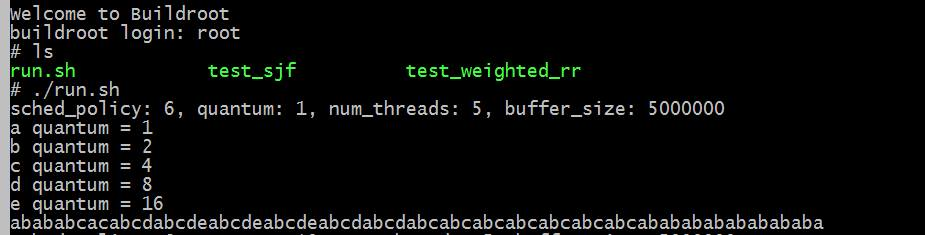
\includegraphics[width=400pt]{images/exp-weighted-rr.jpg}
        \caption{\lstinline{test_weighted_rr.c} 執行結果}
        \label{fig: result}
    \end{center}
\end{figure}

\begin{figure}
    \begin{center}
        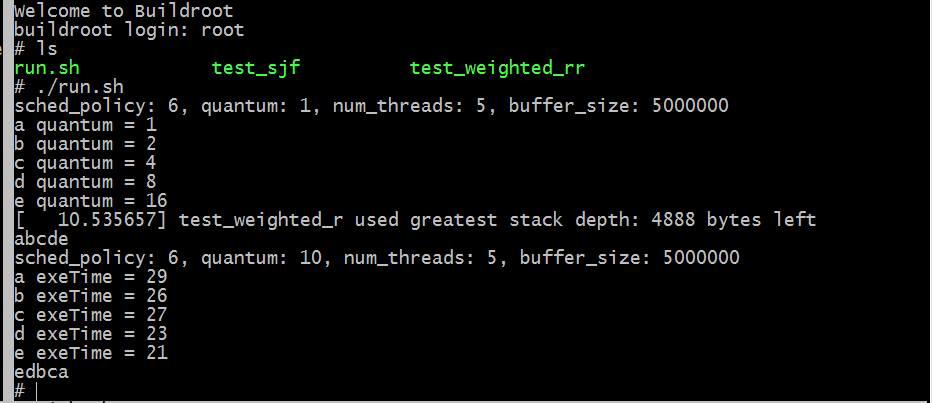
\includegraphics[width=400pt]{images/exp-sjf.jpg}
        \caption{\lstinline{test_sjf.c} 執行結果}
        \label{fig: result}
    \end{center}
\end{figure}

\begin{figure}
    \begin{center}
        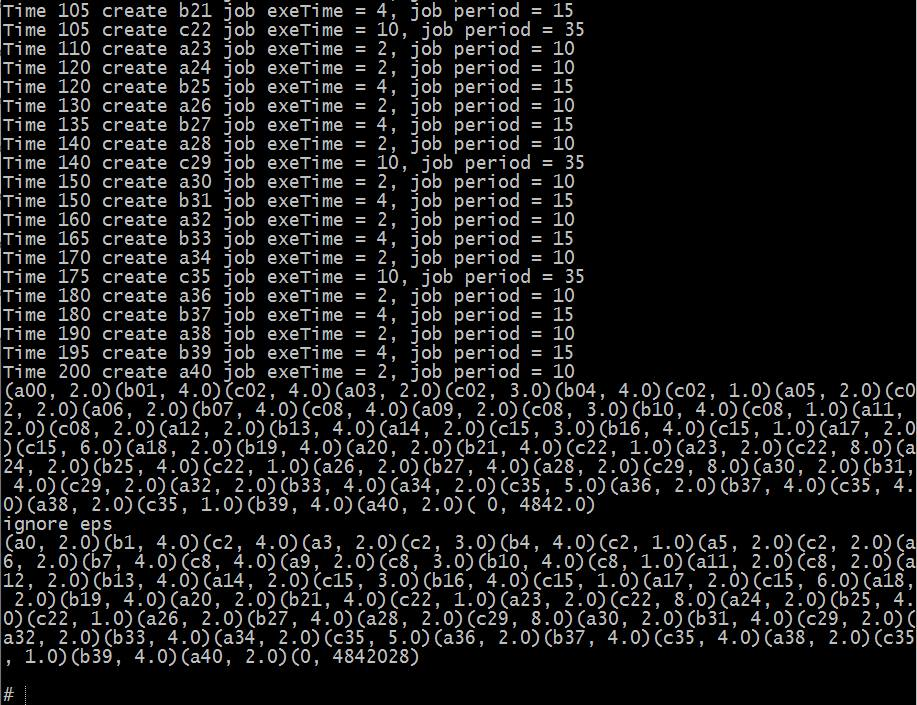
\includegraphics[width=400pt]{images/exp-rms.jpg}
        \caption{\lstinline{test_rms.c} 執行結果}
        \label{fig: result}
    \end{center}
\end{figure}

\vspace*{.1in} \noindent {\large \bfseries Special Thanks}

\begin{itemize}
    \item Lab 332 Parallel and Distributed Laboratory
\end{itemize}

\end{resume}

\end{document}